\documentclass[bg, manuscript]{copernicus}

\usepackage{booktabs}
\usepackage{textcomp}
\usepackage{caption}

\begin{document}

\title{Radiocarbon and thermal fractionation reveal decoupled nitrogen and carbon persistence in soil organic matter: A modeling study of a long-term agricultural trial in Sweden}

% \Author[affil]{given_name}{surname}

\author[1]{Teneille Nel}
\author[2]{Carlos Sierra}
\author[3]{Marie Spohn}

\affil[1]{University of Antwerp, Groenenborgerlaan 171, 2020 Antwerp, Belgium}
\affil[2]{Max Planck Institute for Biogeochemistry, Hans-Knöll-Straße 10, 07745 Jena, Germany}
\affil[3]{Swedish University of Agricultural Sciences, Gerda Nilssons väg 5, 756 51 Uppsala, Sweden}

\correspondence{Teneille Nel (teneille.nel@uantwerpen.be)}
\runningtitle{Decoupled N and C persistence in agricultural soil}
\runningauthor{T. Nel et al.}


\received{}
\pubdiscuss{} %% only important for two-stage journals
\revised{}
\accepted{}
\published{}

%% These dates will be inserted by Copernicus Publications during the typesetting process.


\firstpage{1}

\maketitle



\begin{abstract}
Soil organic matter (SOM) persistence is a key control on terrestrial carbon cycling, yet the extent to which carbon (C) and nitrogen (N) share similar stabilization pathways remains unresolved. Here, we investigated whether the age distributions of C and N diverge across SOM pools in long-term cultivated temperate cropland soils in Sweden. We combined thermal fractionation, elemental analysis, radiocarbon ($\Delta^{14}$C) measurements, and compartmental modeling to quantify differences in C and N persistence. Thermostable SOM fractions contained progressively older C and were systematically enriched in N, with C:N ratios declining significantly across the age continuum relative to bulk soil. This empirical divergence demonstrates that long-term C and N persistence are decoupled in agricultural soils, likely driven by selective stabilization of N-containing compounds on mineral surfaces. Conventional decomposition-only models failed to simultaneously reproduce observed SOC stock declines and $\Delta^{14}$C dynamics without an additional non-respiratory loss pool. Although this lateral C export represented a minor fraction ($< 0.5\%$) of annual decomposition flux, its cumulative effect over decadal timescales was critical for closing the mass balance. Together, these findings demonstrate that persistent SOM dynamics are governed by a combination of selective stabilization, transfer efficiency, and non-respiratory loss processes, emphasizing the need for next-generation SOM models to explicitly represent mineral-associated N controls alongside lateral C transport.
\end{abstract}


\introduction  %% \introduction[modified heading if necessary]
While carbon (C) and nitrogen (N) cycling are fundamental to soil fertility, the extent to which their cycling rates are synchronised within soil organic matter (SOM) remains insufficiently resolved. These elements are often assumed to be tightly coupled, with storage and turnover governed primarily by microbial processes such as mineralization and immobilization, as well as plant physiological controls \citep{Brust2019,Luo2026}. As core constituents of SOM, they regulate ecosystem productivity and nutrient availability \citep{Ma2023}. Nitrogen availability can constrain long-term C sequestration \citep{Luo2006}, yet the mechanisms governing long-term N persistence in soils remain poorly constrained \citep{Luo2026}.

Beyond biological controls, increasing evidence highlights strong abiotic regulation of SOM persistence through mineralogy and organo-mineral interactions. Soil type explains substantial variation in C:N ratios across regions \citep{Ma2023}, suggesting that mineralogical context influences both C and N stabilisation. With progressive decomposition, SOM tends to become relatively N-enriched due to preferential microbial C loss \citep{Xu2013}. Because of functional group chemistry, organic N compounds may exhibit enhanced sorption to mineral surfaces, a process strongly modulated by mineral surface chemistry, pH, oxide crystallinity, and dynamic rhizosphere or competitive anion environments \citep{Kleber2021,Spohn2024,Keiluweit2015}. Preferential N enrichment in mineral-associated organic matter (MAOM) has therefore been proposed to explain higher N contents in fine-textured soils \citep{Spohn2020, Spohn2024}. Sorption of these N-containing compounds can counteract mineralisation and enhance SOM persistence \citep{Hemingway2019, Schmidt2011}, suggesting that mineral-associated stabilisation may exert long-term control over stoichiometry \citep{Koven2013}, yet this is not explicitly represented in many first-order SOM models.  

Conceptually, SOM is often partitioned into active and passive pools with contrasting turnover rates \citep{Paustian1992}. The active pool consists of labile compounds such as dissolved organic matter and particulate organic matter (POM), which responds rapidly to management and drives nutrient cycling \citep{Leuthold2023,Brady2017,Samson2020}. In contrast, passive SOM is stabilised through aggregation and mineral association, forming MAOM \citep{Dynarski2020, Trumbore1996}. MAOM is typically enriched in microbially processed compounds, and its formation is now considered central to long-term SOC persistence \citep{Cotrufo2013, Kallenbach2016, Lavallee2020}. 

Because SOM components decompose at different rates, representing SOC as a single homogeneous pool can bias predictions of long-term dynamics \citep{KgelKnabner2008, Trumbore2009}. Multi-pool representations are therefore essential. Thermal fractionation has emerged as a promising approach to isolate SOM pools based on thermal stability, providing improved constraints on persistence relative to physical fractionation methods \citep{Sanderman2020, Stoner2023}. Radiocarbon ($^{14}\text{C}$), particularly the atmospheric bomb spike, provides a powerful tracer for constraining SOC turnover and transit times when combined with compartmental modelling \citep{Trumbore2009, Torn2009, Sierra2018a, Sierra2018b}. However, equifinality in multi-pool models means that parameter identifiability must be evaluated alongside uncertainty, motivating Bayesian approaches that integrate prior knowledge with probabilistic inference \citep{Wang2013}.

Despite evidence for preferential stabilisation of N-containing compounds, it remains unknown whether C and N diverge in their long-term persistence in field soils. Such decoupling would have important implications for SOM persistence and nutrient limitation. Although MAOM formation is increasingly recognized as a dominant control on long-term SOC storage, there remains a crucial lack of field-based evidence resolving whether C and N share common stabilisation pathways or exhibit decoupled persistence under realistic management conditions. Addressing these knowledge gaps requires integrated field-based evidence that explicitly resolves C and N persistence within mineral-associated and thermally defined SOM fractions.

The objective of this study was to quantify the ages of C and N in SOM in temperate agricultural soils. We tested the hypothesis that older SOM fractions are enriched in N relative to C compared to younger fractions, indicating that N-containing compounds are preferentially stabilized during long-term SOM turnover. To achieve this, we analyse temporal changes in organic C and N across four sites, forming a high-frequency dataset spanning approximately 60 years of continuous observation. The study uses the Swedish long-term Soil Fertility Experiments (1957--1969) \citep{Carlgren2001} which provide a rare opportunity to assess how long-term agricultural practices shape SOM storage and stabilisation. By integrating SOC thermal fractionation, elemental concentrations, and $^{14}\text{C}$ measurements into compartmental SOM models, we quantify C and N fluxes through pools with distinct cycling rates to derive age and transit-time distributions of C and N in agricultural soils. This approach provides a mechanistic constraint on SOM persistence and improved empirical grounding for model parameterisation of long-term C and N dynamics.

\section{Methods and materials}

\subsection{Site and sampling}
The field experiment is replicated at four sites with contrasting soil properties (Tables \ref{table:site} and \ref{table:soilproperties}). Three of the sites are located in the south of Sweden and one of them in central Sweden. In southern Sweden, the experiment started in 1957 and in central Sweden, the experiment started in 1966. The experiment comprises many fertilization treatments \citep{Carlgren2001}, and each plot of the experiment has a size of 125~$\text{m}^2$ at all sites. Here, we studied only the control treatment that does not receive any fertilizer inputs.

At all sites, crop are grown in rotation. In South Sweden, the crop rotation consists of the following crops grown in the following order: spring barley (\textit{Hordeum vulgare} L.), oil seed (\textit{Brassica napus} L.), winter wheat (\textit{Triticum aestivum} L.), and sugar beet (\textit{Beta vulgaris} L.). In central Sweden, the crop rotation consists of the following crops grown in the following order: spring barley, oat (\textit{Avena sativa} L.), oil seed, winter wheat, oat, and winter wheat (winter wheat and oat are grown twice in this rotation). The experiment is maintained by the Swedish University of Agricultural Sciences (SLU) and has the number R3-9001.

Soil samples were collected from all treatments at a soil depth of 0--20~cm at a regular basis (every 3 to 8 years until the year 2019 for this study) right before fertilizer application.

\subsection{Soil chemical analyses and fractionation}

\subsubsection{Soil organic matter fractionation}
All soil samples were dried to constant weight at 35\,$^\circ\text{C}$ (which is a common drying temperature for forest soils and has been the drying temperature of the Swedish National Forest Inventory for the last decades). The dry soil samples were homogenized and sieved ($< 2$\,mm) and roots were removed.

We conducted a ramped thermal fractionation to isolate two SOM fractions. We chose the temperatures for the SOM fractions to be 325\,$^\circ\text{C}$ and 400\,$^\circ\text{C}$ according to the results of previous studies \citep{Sanderman2020, Stoner2023}. The two SOM fractions that differ in thermostability were obtained in two separate thermal fractionations (up to different temperatures) based on two subsamples of one soil sample. Prior to the fractionation, all soils were ground using a ball mill. For the fractionation, 1.6~g of soil was exposed to a ramped temperature treatment in a furnace ventilated with ambient air (Nabertherm with temperature controller C19) with an increase in temperature of 5\,$^\circ\text{C}$ per minute until either 325\,$^\circ\text{C}$ or 400\,$^\circ\text{C}$ were reached. Subsequently, the samples were cooled down at room temperature.

\subsubsection{Soil pH, carbon and nitrogen measurement}
The soil pH was determined in water (at a soil:water ratio of 1:3) using a Pt electrode (Aquatrode Plus Pt1000, Metrohm). The total organic C (TOC) and total N concentrations of the bulk soils and soil fractions were analyzed using an elemental analyzer (TruMac CN, LECO). We also determined the inorganic N of all soils and soil fractions and calculated the total organic N (TON) as the difference between the total N and the total inorganic N. The main purpose of the inorganic N measurement was to confirm that the inorganic N that is formed by the combustion of organic N during the ramped thermal fractionation does not remain in the sample. Inorganic N was extracted in 2.0~M KCl and determined using an autoanalyzer (Seal Analytical). In the thermostable SOM fractions, no inorganic N was detected. The detection limit of the inorganic N quantification is $0.05\,\text{mg N l}^{-1}$, which corresponds to $0.0004\,\text{mg N g}^{-1}$ soil. We calculated the molar TOC:TON ratio, based on the moles of organic C and organic N.

\subsubsection{Statistical comparisons}
The relationship between bulk SOM C:N ratios and SOM age was assessed using ordinary least squares linear regression, with reconstructed system C:N ratios as the response variable and $\log_{10}$-transformed SOM age as the predictor to account for the nonlinear decline of C:N ratios across the age continuum. Differences in C:N among fast-, intermediate-, and slow-cycling pools were assessed using a Friedman test because pool-specific values were paired within sites and sample size was small ($n = 4$).

\subsection{Radiocarbon analyses}
The $\Delta^{14}\text{C}$ of the bulk soils and soil fractions was analyzed using a MIni CArbon DAting System (MICADAS, Ionplus, Dietikon, Switzerland) at the Max Planck Institute for Biogeochemistry in Jena, Germany. Soils contained a small amount of inorganic carbon (an average 0.037\%), which was removed during sample preparation prior to $^{14}\text{C}$ analysis using HCl.

The radiocarbon ratio is reported as $\Delta^{14}\text{C}$ in per mille [\permil], which is the $^{14}\text{C}:^{12}\text{C}$ ratio of the sample with respect to the $^{14}\text{C}:^{12}\text{C}$ ratio of the standard (oxalic acid standard SRM-4990C; \citet{Steinhof2017}) including the normalization for $\delta^{13}\text{C}$ (fractionation correction) and the correction for the decay between 1950 and the measurement time \citep{Stuiver1977}. Positive $\Delta^{14}\text{C}$ values indicate incorporation of bomb-radiocarbon produced by nuclear-bomb tests in the 1950s and 1960s. Negative values indicate that carbon entered the soil before the 1950s and enough time has passed for substantial radioactive decay to occur. The lower the $\Delta^{14}\text{C}$ values, the longer the carbon persisted on average since the time of fixation from the atmosphere.

\subsection{Soil organic matter decomposition modeling}

\subsubsection{Data preparation and aggregation}
All data processing and calculations were performed in R version 4.5.1. SOC stocks were calculated from SOC concentrations using a constant bulk density ($2$) and fixed sampling depth (0.2~m). The mean and standard deviation of SOC stocks and $\Delta^{14}\text{C}$ values were calculated using base R and the \texttt{dplyr} package for datasets aggregated by sampling year and fraction (bulk, 325\,$^\circ\text{C}$ and 400\,$^\circ\text{C}$ thermal fractions), where the 400\,$^\circ\text{C}$ pool was defined as the slow pool.

These summary statistics were also calculated for an intermediate pool (calculated as the difference between 325\,$^\circ\text{C}$ and 400\,$^\circ\text{C}$ fractions) and a fast pool (bulk $-$ 325\,$^\circ\text{C}$ fraction) to form the observational constraints used in model calibration. Uncertainties for derived pools (fast and intermediate) were calculated using quadratic error propagation in base R, assuming no covariance between the uncertainties of contributing fractions.

\subsubsection{Model structure}
SOC dynamics were represented using a compartmental model with three SOM pools connected in series (consecutive transfers from fast- to intermediate- to slow-cycling pools), implemented with the \texttt{SoilR} package \citep{Sierra2012}. Preliminary data investigation revealed a discrepancy between radiocarbon and C stocks data that could only be explained by additional export of SOC besides decomposition, therefore a fourth "loss" pool was incorporated into the model structure. The loss pool represents a pool outside the soil that contains all C that has been lost from the soil by processes other than respiration, such as erosion, leaching, or colloidal transport.

SOC transfers between pools were defined through a decomposition matrix $\mathbf{A}$, parameterized by first-order decay rates and transfer coefficients. These were defined as $k_f$, $k_i$, $k_s$ (decomposition rates of fast, intermediate and slow pool, respectively, while the loss pool was assigned a very small value i.e., $10^{-9}$ to simulate negligible decomposition) and $\alpha_{21}$, $\alpha_{32}$, $\alpha_{41}$ and $\alpha_{42}$ (fractional transfers from fast to intermediate pool, intermediate to slow pool, fast to loss pool and intermediate to loss pool, respectively). The system of ordinary differential equations was solved in \texttt{SoilR}, simultaneously predicting C mass and $^{14}\text{C}$ signatures in all pools.

The SOM decomposition model assumes time-invariant transfer coefficients and decay rates, neglecting feedbacks between substrate quality, microbial activity, and mineral protection. The additional loss pool represents a conceptual export pathway (e.g. erosion or leaching) rather than an explicit biogeochemical process and is treated as a non-reactive sink. While this helps reconcile SOC stocks and $\Delta^{14}\text{C}$ signatures, it introduces assumptions about irreversible SOC loss that are not independently constrained by the data.

\subsubsection{Model initialization}
Atmospheric $\Delta^{14}\text{C}$ values were obtained from the Northern Hemisphere dataset \citep{Hua2022} and $\Delta^{14}\text{C}$ of the SOM pools were simulated from 1957 to 2019 at monthly resolution.

Initial $\Delta^{14}\text{C}$ values were assigned to the bulk and slow pool based on observed signatures. Initial $\Delta^{14}\text{C}$ of the intermediate pool was defined as a parameterized offset from the bulk, while that of the fast pool was fixed based on preliminary model results. The $\Delta^{14}\text{C}$ of the loss pool was given a value equivalent to that of the fast pool, so as not to contribute to the initial system $\Delta^{14}\text{C}$ balance.

Organic C inputs were prescribed at constant annual flux (rate of 80\,g C m$^{-2}$ y$^{-1}$ selected based on preliminary model results), directed exclusively to the fast pool. Initial pool sizes were estimated from observed SOC stocks in the first year, with SOC stocks in the fast and intermediate pools calculated by subtraction (as described in the Data preparation and aggregation section).

Fixed inputs ignore interannual variability in productivity, management, and residue quality, representing long-term mean C forcing rather than dynamic inputs. As a result, turnover parameters reflect effective rates combining decomposition and input variability, rather than true kinetic constants. This may affect parameter identifiability in multi-pool models due to equifinality.

\subsubsection{Parameter estimation}
Model parameters were estimated using nonlinear optimization via the \texttt{FME} package version 1.3.6.4 (\texttt{modCost} and \texttt{modFit} functions). A cost function was defined as the weighted sum of squared residuals between model outputs and observations, normalized by observational uncertainty. The cost function included bulk, fast, intermediate and slow pool SOC stocks, as well as bulk $\Delta^{14}\text{C}$ values. This multi-objective calibration ensured that both SOC stocks and $^{14}\text{C}$ dynamics were simultaneously constrained. Attempts to incorporate $\Delta^{14}\text{C}$ values of the 325 and 400\,$^\circ\text{C}$ thermal fractions as pools containing fast or intermediate fractions in ‘nested’ models, did not result in satisfactory performance and thus $\Delta^{14}\text{C}$ values of thermal fractions were not utilized further in models of this study.

Optimization was performed using the Nelder-Mead algorithm with bounded parameter space. Initial parameter ranges for pool decomposition rates and C transfer coefficients were informed by established multi-pool radiocarbon modeling literature \citep{Gaudinski2000, Manzoni2009, Jenkinson1990, Parton1987}. Site-specific initializations, including the intermediate pool radiocarbon offset ($\text{F}_{0\text{ib}}$) and minor loss coefficients were constrained through exploratory runs and constraints were imposed to ensure physically meaningful values (e.g. positive decay rates, transfer coefficients between zero and one and realistic $\Delta^{14}\text{C}$ ranges). The model returned time series of SOC stocks and $\Delta^{14}\text{C}$ values of bulk soil and SOM pools that were simulated based on the combination of parameters that minimized prediction error compared to the observed data.

\subsubsection{Parameter uncertainty estimation by Bayesian analyses}
To confirm the robustness of inferred SOC turnover dynamics, parameter uncertainty and identifiability were further assessed using a Markov Chain Monte Carlo (MCMC) approach. The MCMC analysis was implemented using the \texttt{FME} package version 1.3.6.4 (\texttt{modMCMC} function) and sampled from the posterior parameter space based on the likelihood defined by the model--data misfit. The likelihood function was derived from the same weighted least-squares cost function used in deterministic calibration, where residuals were normalized by observational standard deviations. Initial parameter values were those of the optimized solution from \texttt{modFit}.

The MCMC was run for 50\,000 iterations and implemented an adaptive Metropolis algorithm combined with a delayed rejection procedure as acceptance criterion \citep{Laine2008}. Parameter bounds were enforced to maintain physically meaningful values. The resulting MCMC chains were analyzed to evaluate parameter uncertainty, covariance and the degree to which parameters are constrained by the data. Marginal posterior distributions were estimated by kernel density estimation, allowing visualization of parameter probability distribution curves derived from MCMC samples. Correlation scatterplots of sampled parameter pairs and trace plots (time series of parameter values across MCMC iterations) were visualized to assess mixing behaviour (efficiency of exploration of parameter space) and stationarity (convergence to target distribution).

Uncertainty in parameter estimations was propagated into model predictions by running the SOC dynamics model across ensembles of parameter sets randomly sampled from the posterior distribution. This produced distributions of SOC stocks and $\Delta^{14}\text{C}$ values from which model prediction uncertainty could be derived.

\subsubsection{Soil organic matter age and transit time}
The age and transit time distribution of bulk SOC as well as pool-specific transit time distributions were derived from the calibrated compartmental model using \texttt{SoilR} functions (\texttt{systemAge} and \texttt{transitTime}) that operate on compartmental matrices constructed using decomposition rate constants, transfer coefficients and C inputs. The analyses were restricted to the active three-pool structure (fast, intermediate and slow), excluding the fourth loss pool, which represents effectively irreversible export with negligible turnover.

System and pool ages and pool transit times were computed for multiple parameter sets over a continuous age domain ranging from 0 to 500 years. The parameter sets were obtained by sampling parameters from the MCMC output to propagate posterior parameter uncertainty. Uncertainty in age and transit time distributions was quantified by aggregating densities across all sampled parameter sets, and 95\% confidence envelopes were calculated. Summary statistics (mean, median and quantiles) for each distribution were computed using density-weighted integrals.

\subsubsection{Age-weighted carbon and nitrogen stock distributions}
Age distributions of SOM were derived by combining age density functions with pool-specific SOC stocks. The SOC stocks of bulk soil and SOM pools were extracted from the final simulation time-step of the best fit parameterisation of the fitted multi-pool decomposition model. The probability density functions of $\text{C}_{\text{age}}$ for each pool were scaled by the C stocks of the respective pools to obtain stock-weighted age distributions. Nitrogen stock distributions were subsequently derived by assuming a constant bulk C:N ratio (confirmed visually in Fig. \ref{fig:fig1}), using the final observed value. Uncertainty in age-weighted stock distributions was quantified using the full ensemble of accepted MCMC parameter sets, producing an ensemble of stock-weighted age distributions for both C and N. Empirical 95\% confidence intervals were calculated across the ensemble for each pool, for both C and N. The median age was calculated for both C and N as the age at which the cumulative distribution reached 50\% of the total stock. Mean C and N ages were computed as the first moment of their respective stock-weighted age distributions, taking the weighted average of age where the weighting factors were the age-specific stock densities.

\subsubsection{Carbon fluxes}
Steady-state carbon fluxes among soil organic matter SOM pools were calculated for each posterior model realization using the estimated pool sizes and kinetic parameters from the radiocarbon-constrained SOM model. Decomposition fluxes were calculated as the product of the pool-specific decomposition rate constants and corresponding C stocks at the final model timestep. Transfer fluxes from fast to intermediate SOM and intermediate to slow SOM pools were calculated by multiplying decomposition fluxes by the estimated transfer coefficients. Export fluxes representing non-respiratory C loss from the modeled SOM system were calculated similarly using the loss coefficients. Respiration fluxes were calculated as the residual fraction of decomposition after accounting for stabilization and export pathways. For each posterior realization, C allocation efficiencies were calculated as the proportion of decomposed C assigned to each pathway (respiration, stabilization, or export) by dividing the respective flux by total pool-specific decomposition. Fluxes and efficiencies were summarized across the posterior parameter distributions using the median and 5th--95th percentiles.

\section{Results}

\subsection{Soil physicochemical properties}
The soil TOC and TON contents varied among the four sites, and they decreased at all four sites over time (Fig. \ref{fig:fig2}). From the first to the last measurement, the TOC content decreased by 35\%, 37\%, and 26\% in the experiments M2, M4 and M6, and the TOC decreased by 25\% in experiment R96 since 1971.

Despite differences in soil C and N across sites, similar trends in C:N ratios justifies our approach of modeling the sites together. The fractions thermostable at 325\,$^\circ\text{C}$ and 400\,$^\circ\text{C}$ contained a larger percentage of the soil TON than of the soil TOC. Hence, the TOC:TON ratios of the thermostable fractions were very low. Specifically, the median TOC:TON ratios in the fraction thermostable at 325\,$^\circ\text{C}$ at the four sites across all sampling times were 5.8, 6.9, 7.4, and 5.8, while the median C:N ratios in the fraction thermostable at 400\,$^\circ\text{C}$ were 4.3, 5.5, 5.2, and 4.1, at the four sites (Fig. \ref{fig:fig2}).

Thermal fractionation generally isolated SOM pools with progressively lower $\Delta^{14}\text{C}$ values, indicating increasing apparent age with increasing thermal stability (Fig. \ref{fig:fig2}). Across all sites, mean $\Delta^{14}\text{C}$ values declined systematically from bulk soil to the 325\,$^\circ\text{C}$ fractions (shifts ranging from $-13$\,\permil{} to $-181$\,\permil{} across sites) and from the 325\,$^\circ\text{C}$ to the 400\,$^\circ\text{C}$ fractions (shifts ranging from $-23$\,\permil{} to $-215$\,\permil{} across sites). This common pattern suggests that thermal fractionation effectively separated SOM into fractions with progressively greater apparent ages across contrasting long-term experimental sites.

\subsection{Model results}

\subsubsection{Temporal predictions of soil carbon stocks and radiocarbon abundance}
We found that multi-pool SOM models could not simultaneously reproduce observed temporal trends in SOC stocks and $\Delta^{14}\text{C}$ without an additional export mechanism. While SOC stock decline was driven primarily by the fast-cycling pool, this pool’s $\Delta^{14}\text{C}$ signature did not show the expected incorporation of atmospheric bomb $^{14}\text{C}$, particularly in light of the low, stable $\Delta^{14}\text{C}$ maintained by the slow-cycling pool. Incorporating non-respiratory losses reconciled the long-term C mass balance and enhanced model performance (reducing SSR from 131 to 105).

The turnover rate of the intermediate pool ($0.00687\,\text{y}^{-1}$) was more similar to that of the slow-cycling pool ($0.008\,\text{y}^{-1}$) than the fast-cycling pool ($0.05\,\text{y}^{-1}$) (Table \ref{tab:pars}). Transfer fractions from the fast to the intermediate and from the intermediate to the slow pool, were similar ($0.128$). However, since the effective stabilization rate is the decomposition rate multiplied by the transfer coefficient, the effective flux equates to less than 1\% of the intermediate pool per year.

\subsubsection{Model diagnostics}
Trace plots showed a positive correlation between $k_i$ (intermediate pool decomposition rate) and $\alpha_{21}$ (transfer from fast to intermediate pool), ($p = 0.88$) and a negative correlation between $k_s$ (slow pool decomposition rate) and $\alpha_{21}$ ($p = -0.51$) (Fig. \ref{fig:figA1}). Convergence plots confirmed equifinality of most parameters, but less so for $k_i$, $k_s$ and $\alpha_{21}$ (Fig. \ref{fig:figA2}).

Although the posterior distributions for the intermediate-pool radiocarbon adjustment parameter and $\alpha_{42}$ (transfer from intermediate to loss pool) are broad (Fig. \ref{fig:figA1}), their plausible ranges remain relatively narrow, suggesting that both parameters are well constrained. In contrast, the multimodal distribution of $k_i$ indicates some structural non-identifiability.

Confidence intervals (CIs) of predicted SOC stocks and $\Delta^{14}\text{C}$ values were much smaller than the standard deviation of observed measurements (Table \ref{tab:pred} and Fig. \ref{fig:fig3}), supporting the value of models that incorporate data from different sites to reveal overall trends.

\subsubsection{Soil organic matter age and transit time}
Slow SOM pools exhibited broad skewed age distributions extending across centennial timescales (Fig. \ref{fig:figA3}). Narrow uncertainty envelopes for fast pool ages and system transit time reflect strong constraint of rapid cycling processes by the observational data, whereas broader distributions for intermediate and slow pools indicate greater uncertainty in longer-term carbon persistence (Fig. \ref{fig:figA3}).

The fast-cycling pool had a mean age (19 years). The cycling rate of the intermediate pool was closer to that of the slow pool than the fast pool. The mean system age (79 years) was skewed right relative to the median system age (35 years). Mean system ages of the fast and intermediate pools were also skewed right relative to their corresponding median ages, while the mean and median ages of the slow-cycling pool were relatively similar.

\subsubsection{Weighted age distributions of soil organic carbon and nitrogen}
C:N ratios decreased systematically across the age continuum, declining rapidly at younger SOM ages and approaching lower values at centennial timescales (Fig. \ref{fig:fig4}; linear regression of C against $\log_{10}$-transformed age: $\beta = -6.42$, $R^2 = 0.82$). C:N ratios differed significantly among operational SOM pools (Friedman test, $\chi^2_{(2)} = 6$, $p = 0.04979$). Fast-cycling pools had substantially higher C:N ratios (mean 22) than intermediate (6.7) and slow pools (4.6). As a result of lower C:N ratio of older pools, the weighted density distribution of bulk N stocks were shifted right compared to C stocks (Fig. \ref{fig:fig5}).

\subsubsection{Carbon pool fluxes}
Fast-cycling SOM dynamics dominated the total SOM flux (Fig \ref{fig:fig6}), with $72.8\,\text{g C m}^{-2}\,\text{y}^{-1}$ respired as $\text{CO}_2$ (Fig. \ref{fig:figA4}). The majority of decomposed carbon was returned to the atmosphere through respiration across SOM pools, with median respiratory fractions of decomposition of 83\% and 91\% for the fast and intermediate pools, respectively (Table \ref{tab:fluxes}). A relatively large proportion (16.7\%) of decomposed fast-pool C was partitioned into intermediate SOM, while only a small proportion (8.0\%) of intermediate C was partitioned into the slow pool. Lateral export represented an almost negligible fraction ($< 0.5\%$) of decomposition flux.

\section{Discussion}

This study demonstrates that soil organic carbon (SOC) and nitrogen (N) in the four cultivated soils studied here do not share the same age distribution. Thermal fractionation and radiocarbon modeling revealed that older SOM fractions were enriched in N relative to C compared to younger fractions, suggesting preferential stabilization of N-containing compounds. Furthermore, the inability of decomposition-only models to reproduce both SOC stocks and $\Delta^{14}\text{C}$ dynamics indicates that non-respiratory C losses are important components of long-term SOC dynamics in agricultural systems.

\subsection{Thermal stability reveals systematic differences in SOM age and C:N stoichiometry}  
Our result that N-containing compounds are preferentially retained in persistent SOM fractions compared to more labile fractions supports our hypothesis that older SOM fractions are enriched in N relative to C compared to younger fractions. The finding is supported by previous studies reporting preferential adsorption of N-containing compounds to mineral surfaces \citep{Cao2011, Kopittke2018, Daly2021}. Because amino acids and peptides contain both amino and carboxyl functional groups, they may form stronger mineral associations than many N-free organic compounds \citep{Spohn2024}. This may lead to disproportionate retention of organic N within persistent SOM pools and contribute to divergence between the age distributions of C and N observed in SOM fractions.

Proteins, particularly globular proteins, readily interact with mineral surfaces through a combination of hydrophobic interactions, electrostatic forces, ligand exchange, and conformational rearrangements that enhance their adsorption and reduce their accessibility to microbial enzymes \citep{Haynes1994, Yu2002}. Once stabilized on mineral surfaces, proteins can persist for extended periods compared with more labile organic compounds due to reduced desorption and enzymatic accessibility \citep{Demarchi2016}. Because proteins represent a major reservoir of organic N in soils, their enzymatic depolymerization into amino acids is often considered a rate-limiting step in terrestrial N cycling \citep{Jan2009}.

Recent advances in SOM theory highlight that persistent SOM is not solely derived from chemically recalcitrant plant compounds but is strongly shaped by microbial transformation and subsequent stabilization \citep{Liang2019}. Microbial necromass, which is enriched in N-containing compounds such as amino sugars, peptides, and microbial cell wall constituents, represents a substantial fraction of persistent SOM and provides an important pathway for the accumulation of N-rich SOM \citep{Miltner2012}. Following microbial turnover, necromass-derived compounds can become strongly associated with mineral surfaces, reducing decomposition rates and contributing to long-term SOM persistence \citep{Kallenbach2016}.

Nitrogen age distributions in this study were reconstructed from the model-derived carbon age distributions using the observed final C:N ratio of each modelled C pool, assuming that N shares the same age distribution as C within each pool and that C:N remains constant across that distribution. This assumption is likely reasonable for the slow pool, and potentially also for the intermediate pool, given their low C:N ratios, which suggest that most C is associated with N-containing compounds. In contrast, it may be less appropriate for the fast pool, which has a higher C:N ratio and therefore contains a greater proportion of N-free structural compounds. These compounds may decompose at different rates from labile N-bearing compounds such as amino acids and proteins, meaning that C and N may not necessarily have identical age distributions within this pool. Nevertheless, because the older intermediate and slow pools have lower C:N ratios than the fast pool, the reconstructed bulk N age distribution shifts toward older ages relative to the corresponding C age distribution.

\subsection{Long-term SOC dynamics reflect processes beyond decomposition}
Post-1960s bulk soil $\Delta^{14}\text{C}$ revealed relatively low incorporation of bomb $\Delta^{14}\text{C}$ compared to sites with smaller SOC stocks \citep{Baisden2013, Stoner2021}. This pattern suggests that larger SOC pools require substantially greater organic inputs to shift their overall isotopic signature. Indeed, \citet{Mills2014} observed a pronounced increase in slow-pool $\Delta^{14}\text{C}$ in a soil with similar C stocks only when input rates were much higher. The requirement for an additional loss pool to reproduce both SOC stocks and $\Delta^{14}\text{C}$ dynamics suggests that decomposition alone was insufficient to explain long-term SOC dynamics in these agricultural soils, suggesting that a portion of recent C inputs is exported via erosion or dissolved organic carbon (DOC) leaching. This finding is consistent with studies showing that processes other than heterotrophic respiration, such as erosion, leaching or colloidal transport can contribute substantially to SOC export over decadal timescales \citep{Berhe2012, Doetterl2016, Quinton2010}. The negligible contemporary export fluxes ($< 0.5\%$ of decomposition) suggest that the additional loss pool inferred by the model represents cumulative long-term lateral C redistribution rather than a dominant annual loss pathway, highlighting how small persistent fluxes can influence centennial-scale SOC and $\Delta^{14}\text{C}$ dynamics. While dedicated soil-geomorphology frameworks incorporate spatial SOC redistribution, standard point-scale 1D decomposition models, which are still widely used in soil C accounting, typically omit these C export pathways. Furthermore, current Earth system model representations typically assume similar turnover kinetics for C and N within conceptual pools despite evidence for preferential N stabilisation \citep{Spohn2024, Koven2013}. Unaccounted model assumptions regarding decoupled kinetics, e.g. absence of erosion, limit confidence in predicting long-term C sequestration potential and coupled climate-soil-nutrient feedbacks under global change \citep{Luo2004, Yu2024, GonzalezSosa2024}. Our results therefore underscore the importance of integrating physical C loss processes and decoupled C-N turnover into mainstream SOC modeling frameworks.

\subsection{SOM persistence reflects slow turnover rather than efficient transfer to increasingly stable pools}
The posterior flux estimates indicate asymmetric carbon transfer among the modelled SOM pools, although this pattern is likely influenced by the thermal fractionation scheme used to define the pools. Most conventional fractionation approaches rely on physical separations that conflate materials of different ages, obscuring true turnover dynamics \citep{Castanha2008}. Thermal fractionation offers a mechanistically grounded alternative by separating SOM according to intrinsic thermal stability \citep{Fernandez2011}, improving the resolution of mineral-associated and chemically protected pools \citep{Sanderman2020, Stoner2023}. However, questions remain regarding what thermally defined loss pools represent mechanistically and how they directly map onto mineral protection, particularly for N-containing compounds and their stabilization mechanisms.

A substantial fraction of decomposition flux from the fast-cycling pool was transferred to the intermediate pool (16.7\%), indicating that younger SOM can contribute to more persistent organic matter. In contrast, transfer from the intermediate to slow pool was lower (8.0\%). However, this difference should not necessarily be interpreted as increasingly strong constraints on the formation of highly persistent SOM, because the intermediate and slow pools had relatively similar age distributions and may partly reflect the way the thermal fractions were defined. Respiration accounted for the majority of decomposition flux across all pools, indicating that SOM persistence primarily reflects slow turnover rather than efficient recycling into progressively older pools.

The short carbon transit times reported by \citet{Spohn2023} for a long-term Swedish agricultural experiment provide an important context for our results. Their two-pool model estimated mean transit times of $< 10$ years, indicating that most incoming C was rapidly respired and that only a small fraction remained in soil for several decades. Our results are consistent with this strong dominance of rapid C loss, with respiration accounting for most decomposition fluxes across the modeled SOM pools. However, the three-pool structure used here provides greater resolution of the fate of the fraction that is retained, revealing progressively less efficient transfer into the most persistent SOM. Thus, the short transit times reported by \citet{Spohn2023} is not necessarily due to an absence of persistent SOM; rather, it indicates that persistence is generated by a relatively small fraction of C that escapes rapid loss and turns over slowly once retained.

\subsection{Fractionation methodology, model uncertainty and implications for interpreting SOM pools}
The mean age of the fast-cycling pool was relatively old, considering that rapid-cycling pools usually have mean ages of a few months to a decade \citep{Trumbore2009}. This may reflect climate-related constraints on decomposition in the boreal region of study, as previous studies of sites with similar climate found similarly low $\Delta^{14}\text{C}$ values of TOC \citep{Spohn2023, Ellert2006}, while higher $\Delta^{14}\text{C}$ values, even before the $^{14}\text{C}$ bomb spike of the 1960s, were reported for sites in more temperate climatic zones \citep{Stoner2021, Baisden2013, Mills2014}. Management-related processes such as accelerated loss of labile C through tillage disturbance may also have contributed to the greater mean age of the fast-cycling pool \citep{Grandy2007}. The relatively similar age distributions of the intermediate- and slow-cycling pools should, however, be interpreted in the context of the thermal fractionation methodology rather than solely as evidence of similar SOM turnover dynamics. Because labile carbon was removed at 325\,$^\circ\text{C}$, which is relatively close to the 400\,$^\circ\text{C}$ treatment defining the slow pool, the intermediate and slow fractions may contain more similar carbon age distributions than would be expected for biologically distinct pools. Consequently, the estimated transfer between these pools may partly reflect the operational fractionation scheme. If the intermediate pool were larger or more clearly differentiated in age from the slow pool, the inferred transfer dynamics could differ.

The positive correlation between $k_i$ and $\alpha_{21}$ and negative correlation between $k_s$ and $\alpha_{21}$ indicate trade-offs between decomposition and transfer processes. The lower degree of convergence for $k_i$, $k_s$, and $\alpha_{21}$ suggests that multiple combinations of these parameters can explain the observed SOC dynamics, reflecting uncertainty in partitioning C fluxes among intermediate and slow pools.

\subsection{Implications for C-N coupling and long-term SOM stabilization}
From an agroecosystem perspective, the results of our study imply that long-term management may differentially affect soil C and N retention. Preferential stabilisation of N in mineral-associated fractions could partly buffer soil N losses under continuous cultivation, but may also contribute to declining N availability for plant uptake if strongly protected pools become less accessible. Conversely, management practices that enhance physical disturbance or reduce mineral protection (e.g. intensive tillage) may accelerate both C and N losses, but not necessarily in proportion, potentially altering soil fertility stoichiometry over decadal timescales.

Future studies should investigate mechanisms of selective stabilization of N-containing compounds contributing to long-term persistence of soil organic N in agricultural soils, particularly in different soil types. Variation in mineral composition and chemical conditions among soils could influence the strength and reversibility of organo-mineral interactions, thereby contributing to differences in C and N transit-time distributions. Short-range-order Fe and Al oxides possess high surface charge density and strong affinity for organic ligands \citep{Wang2013}, potentially enhancing retention of N-rich compounds. Rhizosphere acidification and competition with phosphate for sorption sites may promote desorption of mineral-associated SOM \citep{Keiluweit2015, Spohn2022}, thereby increasing accessibility of previously protected organic matter to microbial decomposition.

\conclusions %% \conclusions[modified heading if necessary]
Combining thermal fractionation, $\Delta^{14}\text{C}$ tracking, and compartmental modeling demonstrated that soil organic C and N possess distinct age distributions across the studied cropland soils. More thermostable, longer-persisting SOM fractions were systematically enriched in N compared to less stable SOM fractions, resulting in lower C:N ratios at older age distributions compared to bulk soil. This divergence indicates that selective stabilization, likely via mineral surface binding of N-rich compounds like proteins and microbial necromass, decouples long-term organic N retention from bulk C turnover. Our modeling further revealed that microbial decomposition kinetics alone could not simultaneously reproduce observed long-term SOC stock declines and $\Delta^{14}\text{C}$ dynamics. Reconciling these trajectories required incorporating an additional non-respiratory loss pool. Although this lateral C export represented a small fraction of the annual decomposition flux ($< 0.5\%$), its cumulative effect over decadal timescales significantly impacted mass balances and prevent overestimating the residence time of persistent SOM pools. Standard 1D point-scale models that ignore non-respiratory export pathways risk misattributing physical C losses to heterotrophic respiration. Together, these findings highlight fundamental structural limitations in conventional first-order SOM models that assume uniform C and N turnover or ignore lateral transport. To improve predictions of agricultural soil fertility and carbon cycling, next-generation Earth system and agroecosystem models must explicitly represent mineralogical controls on selective N stabilization alongside physical C export processes such as erosion and DOC leaching.

\dataavailability{Data and code associated with this study are available online \citep{Nel2026}.}

\authorcontribution{T.N. conducted formal analyses, modelling and data visualization and prepared the original manuscript draft. C.A.S. facilitated the radiocarbon analyses, developed modelling packages and assisted in research investigation. M.S. conceptualized the study, was responsible for funding acquisition and project administration and provided supervision. All authors constributed to manuscript review and editing.}

\competinginterests{The authors declare that they have no conflict of interest.}

\begin{acknowledgements}
The authors thank Hui Liu and Anna Oskar for the laboratory work at SLU, and Axel Steinhof for the radiocarbon measurements. M.S. thanks the European Research Council for funding (101043387).
\end{acknowledgements}

\clearpage

%% TABLES
\subsection{Tables}
\clearpage

%%% TABLE 1
  
\begin{table*}[t]
\caption{Location, climate properties and date of initiation (Year) of the four sites. MAT and MAP represent mean annual temperature ($^\circ$C) and mean annual precipitation (mm), respectively. The climate data are derived from the weather stations of the Swedish Meteorological and Hydrological Institute for the periods 1961--1990 and 1991--2020.}
\label{table:site}
\begin{tabular}{lccccccccc}
\tophline
Site & No. & Year & Lat. & Long. & Elev. & MAT & MAT & MAP & MAP \\
 & & & ($^\circ$N) & ($^\circ$E) & (m) & 1961--1990 & 1991--2020 & 1961--1990 & 1991--2020 \\
\middlehline
Orup & M2 & 1957 & 55.82 & 13.50 & 113 & 7.0 & 8.1 & 693 & 755 \\
Örja & M4 & 1957 & 55.73 & 13.05 & 73 & 7.7 & 8.8 & 665 & 676 \\
Ekebo & M6 & 1957 & 55.99 & 12.88 & 72 & 7.6 & 8.7 & 703 & 722 \\
Bjertorp & R94 & 1966 & 58.24 & 13.07 & 80 & 6.1 & 7.3 & 558 & 584 \\
\bottomhline
\end{tabular}
\belowtable{}
\end{table*}

\clearpage

%%% TABLE 2
\begin{table*}[t]
\caption{Soil properties of the soils of the four sites. The chemical soil properties refer to the uppermost 20\,cm of the soils and are means calculated across all treatments and across all years.}
\label{table:soilproperties}
\begin{tabular}{lcccccc}
\tophline
Site name & Soil order & \multicolumn{3}{c}{Texture (\%)} & Bulk density & pH \\
 & & Clay & Silt & Sand & ($\text{g}\,\text{cm}^{-3}$) & \\
\middlehline
Orup & Haplic Phaeozem & 12 & 29 & 59 & 1.51 & 6.1 \\
Örja & Eutric Cambisol & 23 & 25 & 52 & 1.72 & 7.1 \\
Ekebo & Eutric Cambisol & 18 & 35 & 47 & 1.44 & 6.4 \\
Bjertorp & Not determined & 30 & 54 & 16 & 1.37 & 6.4 \\
\bottomhline
\end{tabular}
\end{table*}
\clearpage

%%% TABLE 3
\begin{table}[t]
\caption{Best-fit parameter estimates for the three-pool soil organic matter decomposition model simultaneously fitted to bulk soil organic carbon (SOC) stocks, bulk $\Delta^{14}\text{C}$, and thermally defined fast, intermediate and slow SOC pools across the four long-term agricultural field experiments. Parameters $p_1$--$p_6$ represent $k_{\text{f}}$, $k_{\text{i}}$, $k_{\text{s}}$ (fast, intermediate and slow pool decomposition rates), $a_{21}$ (coefficient indicating proportion of C transfer from fast to slow pool), $F_{0\text{ib}}$ (a value that is subtracted from initial bulk radiocarbon measurement to find the initial intermediate radiocarbon value), $a_{32}$ (transfer coefficient from intermediate to slow pool), $a_{41}$ and $a_{42}$ (transfer from fast and intermediate pools to the ``loss'' pool).}
\label{table:pars}
\begin{tabular}{lc}
\tophline
Par & Value \\
\middlehline
$k_{\text{f}}$ & 0.050671 \\
$k_{\text{i}}$ & 0.00687 \\
$k_{\text{s}}$ & 0.008282 \\
$a_{21}$ & 0.127815 \\
$F_{0\text{ib}}$ & $-3.17351$ \\
$a_{32}$ & 0.127896 \\
$a_{41}$ & 0.003507 \\
$a_{42}$ & 0.005564 \\
\bottomhline
\end{tabular}
\end{table}
\clearpage

%%% TABLE 4
\begin{table}[t]
\caption{Mean observed standard deviation (SD) of measured soil organic carbon stocks and $\Delta^{14}\text{C}$ values, together with the mean half-width of the posterior 95\% confidence interval (prediction error) of model predictions for each soil organic matter pool.}
\label{table:preds}
\begin{tabular}{llcc}
\tophline
Variable & Pool & Observed SD & Prediction \\
\middlehline
C stocks & Bulk & 1699.21 & 129.88 \\
C stocks & Fast & 1812.15 & 74.37 \\
C stocks & Inter & 617.66 & 72.25 \\
C stocks & Slow & 134.19 & 34.43 \\
$\Delta^{14}\text{C}$ & Bulk & 48.84 & 3.64 \\
$\Delta^{14}\text{C}$ & Fast & NA & 2.03 \\
$\Delta^{14}\text{C}$ & Inter & NA & 15.1 \\
$\Delta^{14}\text{C}$ & Slow & 189.63 & 7.48 \\
\bottomhline
\end{tabular}
\end{table}
\clearpage

%%% TABLE 5
\begin{table*}[t]
\caption{Posterior estimates of modeled steady-state carbon fluxes among soil organic matter pools. Values represent the median flux and the 5th and 95th percentiles of the posterior distributions.}
\label{table:fluxes}
\begin{tabular}{llcc}
\tophline
Process & Flux & Median flux & 5--95\% percentile \\
 & & \multicolumn{2}{c}{($\text{g}\,\text{C}\,\text{m}^{-2}\,\text{y}^{-1}$)} \\
\middlehline
Decomposition & Fast pool & 87.8 & 82.7--91.0 \\
Decomposition & Intermediate pool & 10.8 & 8.6--13.0 \\
Stabilization & Fast $\rightarrow$ intermediate pool & 14.7 & 13.0--15.8 \\
Stabilization & Intermediate $\rightarrow$ slow pool & 0.862 & 0.0411--1.88 \\
Respiration & Fast pool & 72.8 & 68.5--76.2 \\
Respiration & Intermediate pool & 9.78 & 6.93--12.6 \\
Respiration & Slow pool & 3.46 & 2.76--4.5 \\
Export & Fast pool & 0.217 & 0.0206--0.71 \\
Export & Intermediate pool & 0.0452 & 0.00303--0.108 \\
\bottomhline
\end{tabular}
\end{table*}
\clearpage
  
\subsection{Figures}

%%fig 1
\begin{figure}[t]
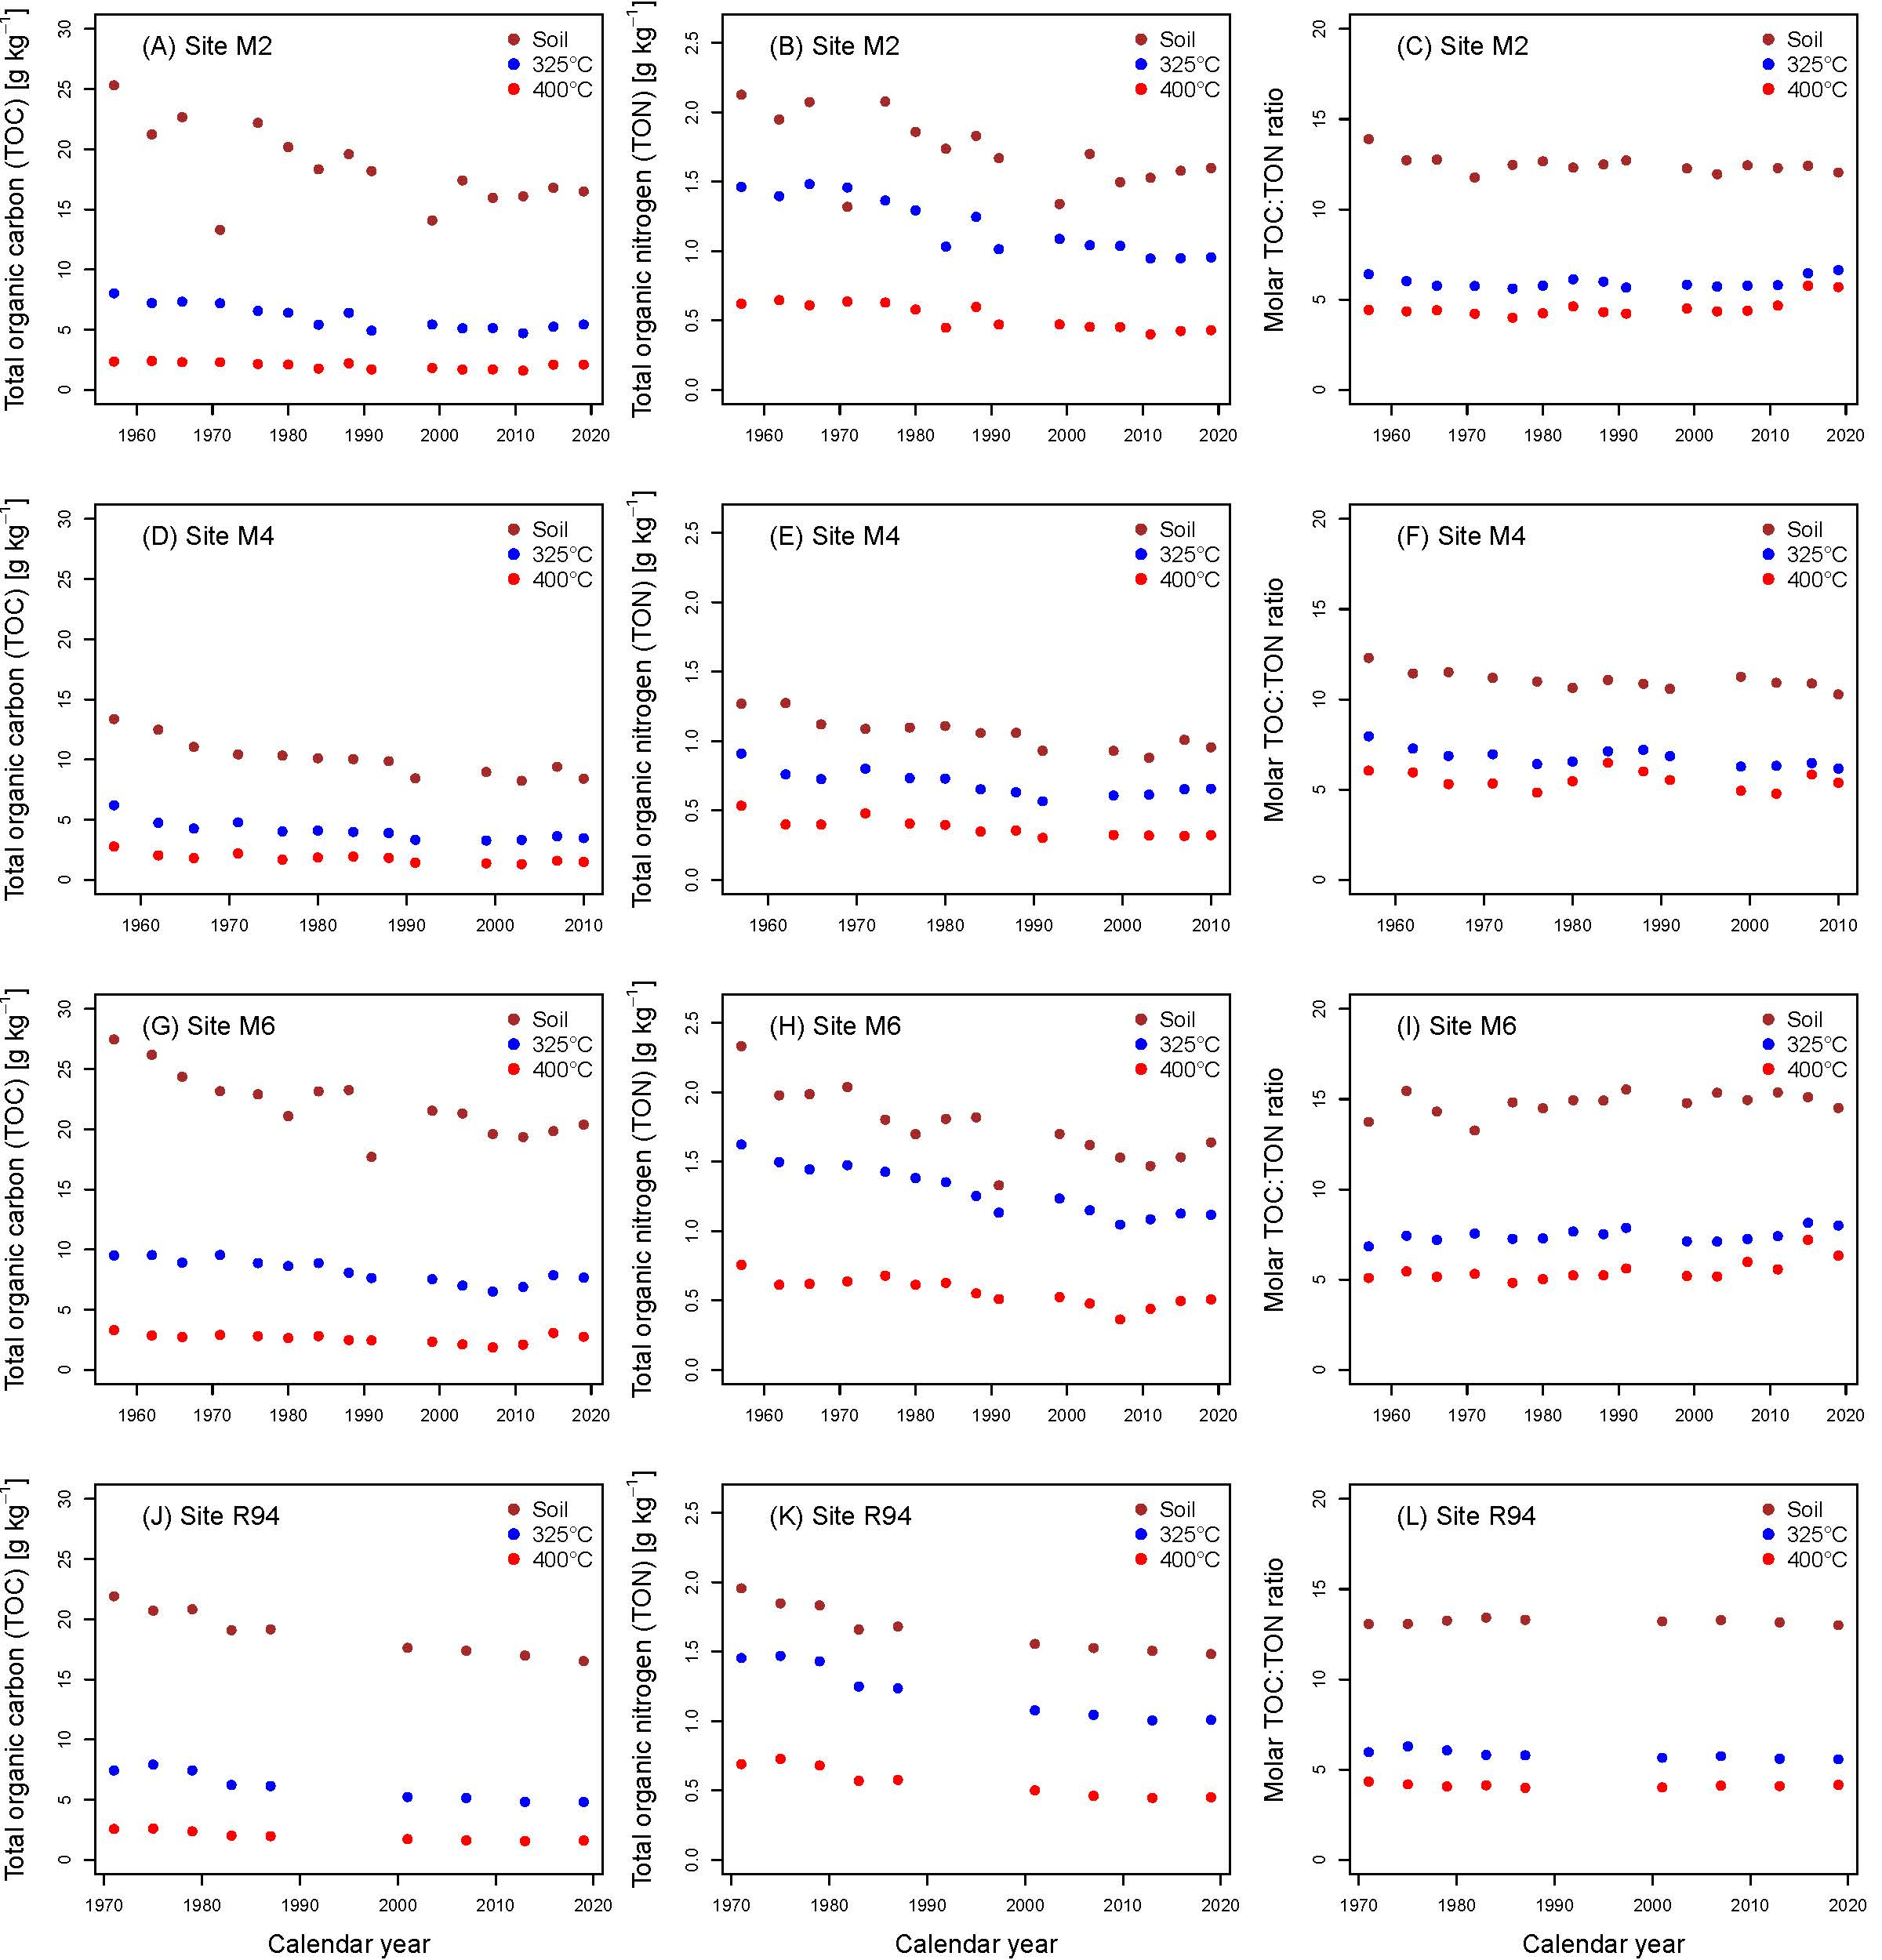
\includegraphics[width=14 cm]{images/tocton.jpg}
\caption{Total organic carbon (TOC), total organic nitrogen (TON), and the TOC:TON ratio in the soils and soil thermal fractions of the four sites (M2, M4, M6 and R96) as a function of time. TOC is shown in panels A, D, G, and J, TON is shown in panels B, E, H, and K, and the TOC:TON ratio is shown in panels C, F, I and L.}
\label{figure:fig1}
\end{figure}
\clearpage

%%fig 2
\begin{figure}[t]
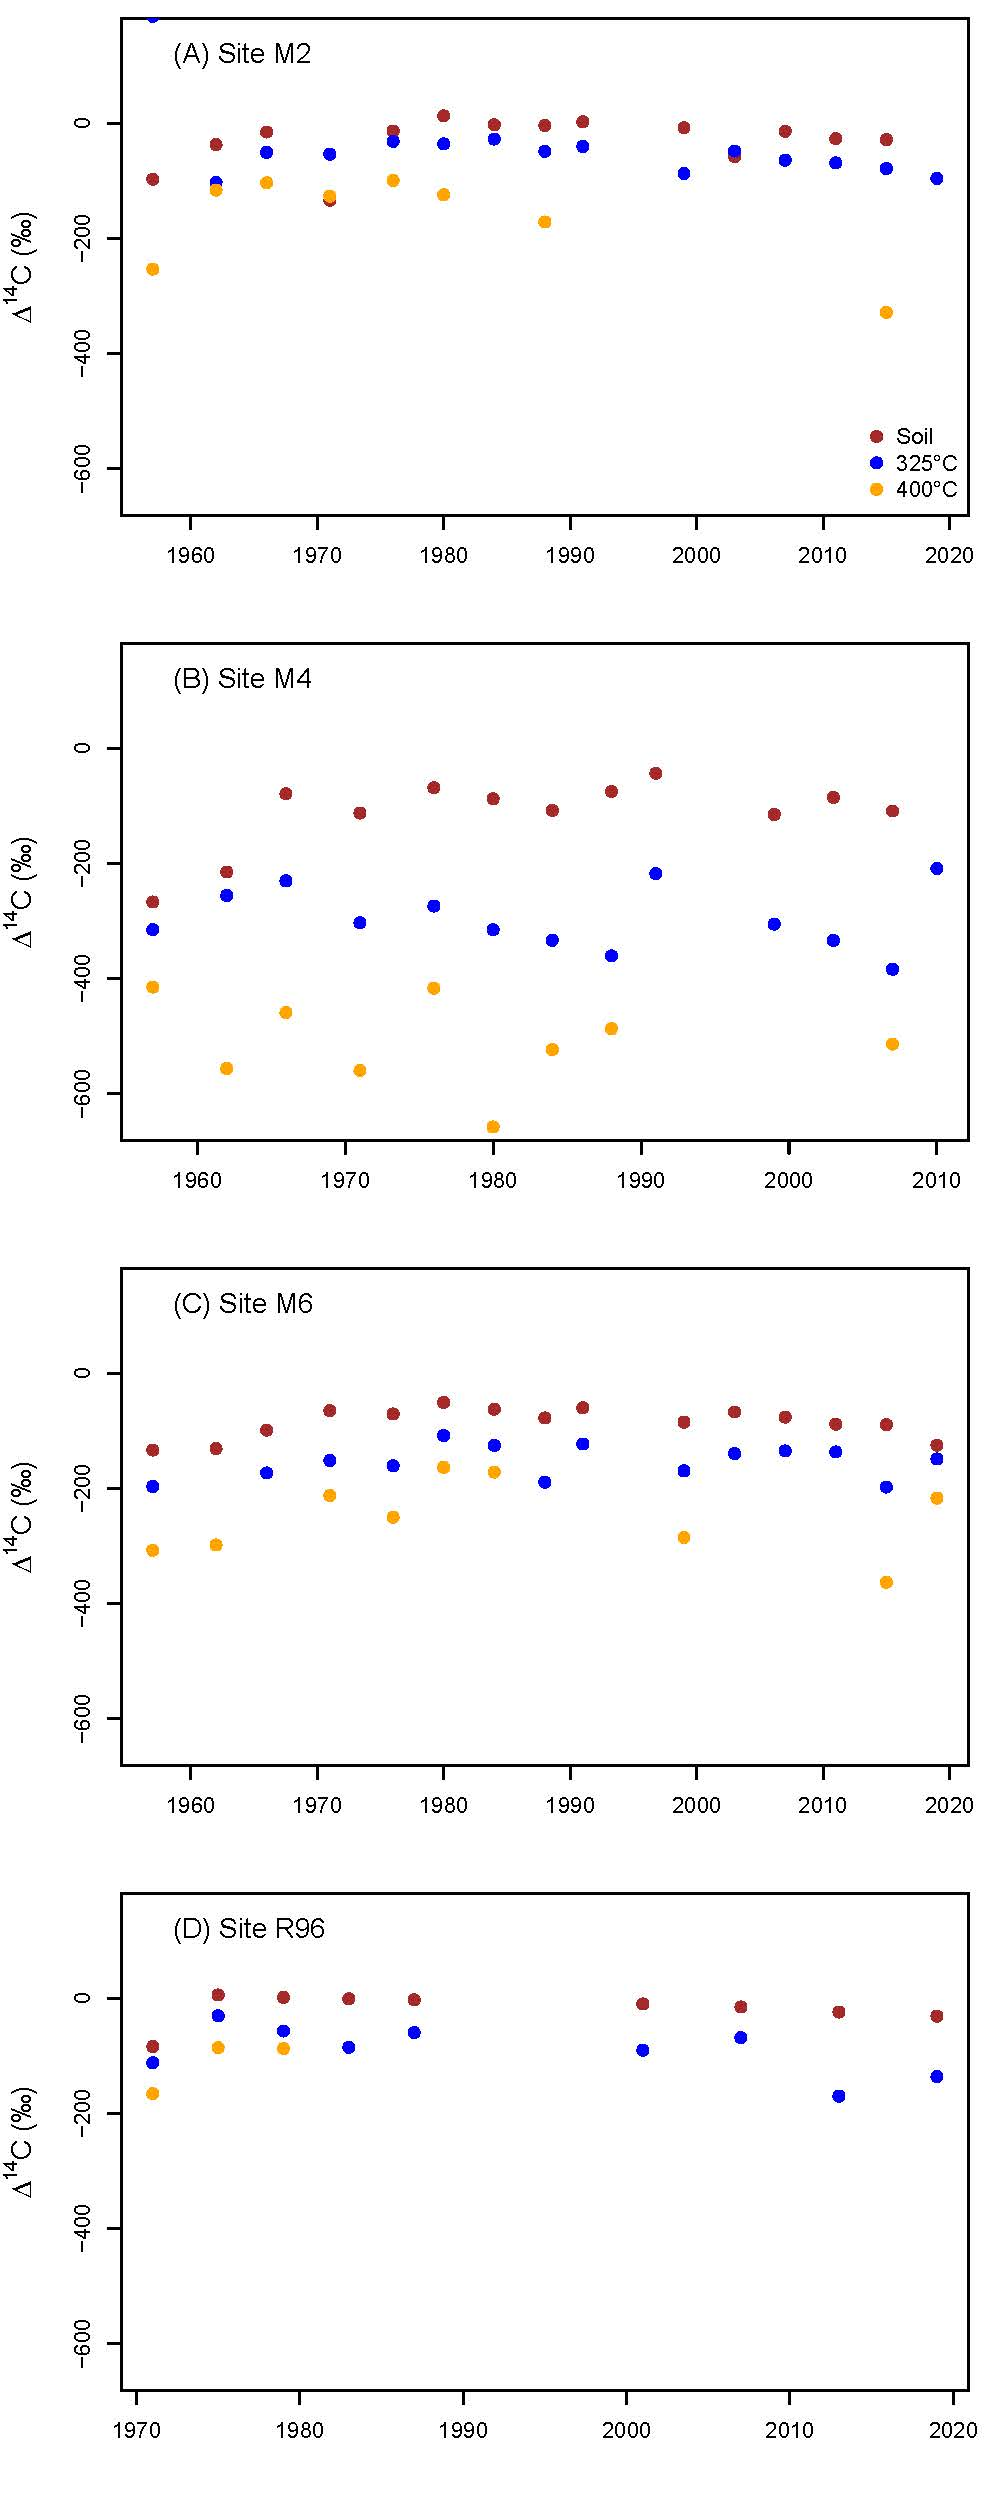
\includegraphics[width=8.3cm]{images/14c.jpg}
\caption{Radiocarbon abundance ($\Delta^{14}$C) in the soils and soil thermal fractions of the four sites (M2, M4, M6 and R96) as a function of time.}
\label{figure:fig2}
\end{figure}
\clearpage
  
%%fig 3
\begin{figure}[t]

\includegraphics[width=11cm]{images/C_and_C14_combined}
\caption{Observed and predicted temporal changes in (A) carbon (C) stocks and (B) radiocarbon abundance ($\Delta^{14}$C) of bulk soil organic matter, three stability pools (fast, inter, slow), and a modeled "loss" pool. Lines and shaded regions represent mean predictions and 95\% confidence intervals, respectively, simulated using a 4-pool, compartmental series structure in SoilR. Model parameters and their associated uncertainties were optimized via Markov Chain Monte Carlo sampling against observed data (points; error bars $\pm$ SD).}
\label{figure:fig3}
\end{figure}
\clearpage

%%fig 4
\begin{figure}[t]

\includegraphics[width=11cm]{images/plot_CN_system}
\caption{Carbon: Nitrogen (C: N) ratio versus age distributions of soil organic matter plotted on a logarithmic axis to capture the wide range of values. Lines and shaded regions represent mean predictions and 95\% confidence intervals, respectively, simulated using a 4 pool, compartmental series structure in SoilR. Model parameters and their associated uncertainties were optimized via Markov Chain Monte Carlo sampling against observed bulk and pool-specific data.}
\label{figure:fig4}
\end{figure}
\clearpage
  
%%fig 5
\begin{figure}[t]

\includegraphics[width=11cm]{images/CN_age_distribution_combined.png}
\caption{Mass-weighted carbon (C) and nitrogen (N) age distributions derived from the best-fit multi-pool model (final timestep), plotted on a logarithmic axis to capture the wide range of values. Age probability densities for bulk soil and soil organic matter (SOM) pools are scaled by their respective C stocks. Nitrogen stocks assume a constant C:N ratio based on final observed values. Mean ages represent mass-weighted averages of C and N across age classes. Lines and shaded regions represent mean predictions and 95\% confidence intervals, respectively, simulated using a 4-pool, compartmental series structure in SoilR. Model parameters and their associated uncertainties were optimized via Markov Chain Monte Carlo sampling against observed bulk and pool-specific data.}
\label{figure:fig5}
\end{figure}
\clearpage

%%fig 6
\begin{figure}[t]
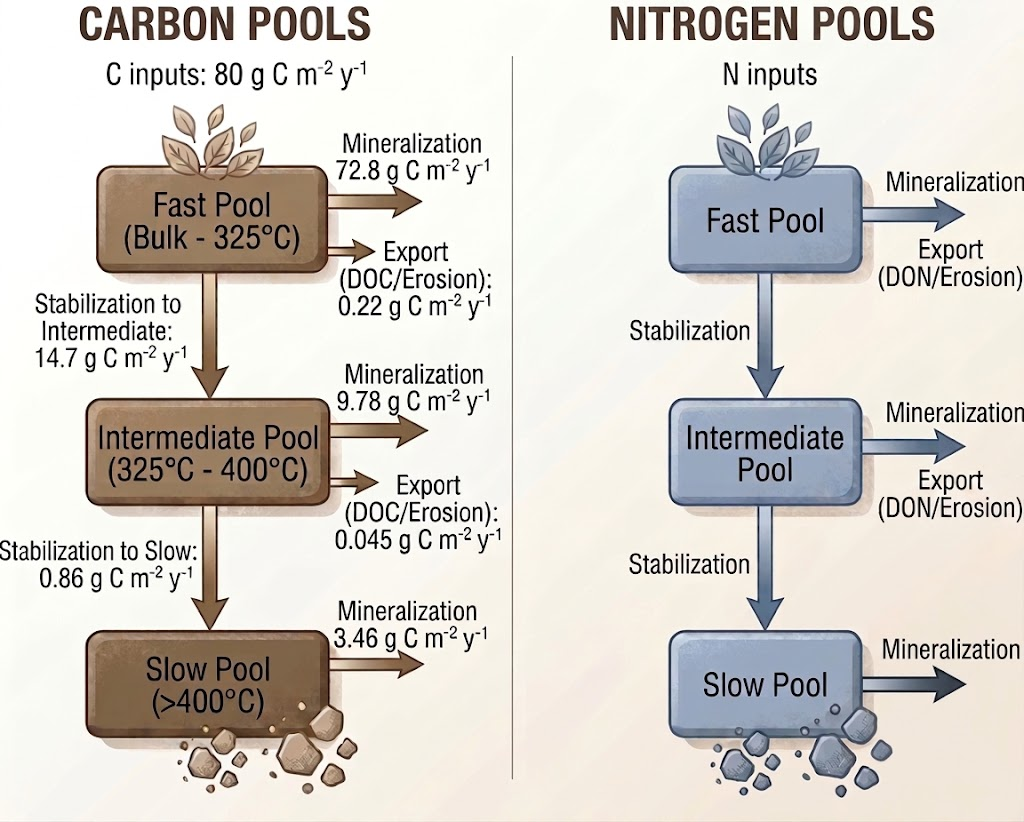
\includegraphics[width=11cm]{images/conceptual.jpg}
\caption{Conceptual diagram showing fluxes of carbon and nitrogen between fast-, intermediate- and slow-cycling soil organic matter pools and the environment.}
\label{figure:fig6}
\end{figure}
\clearpage

\appendix
\section{}    %% Appendix A

%%fig A1
\begin{figure}[t]

\includegraphics[width=11cm]{images/pairs_plot.png}
\caption{Pairwise parameter (p) relationships from the MCMC posterior distribution, where p1--p6 represent $k_f$, $k_i$, $k_s$ (fast, intermediate and slow pool decomposition rates), $a21$ (coefficient indicating proportion of C transfer from fast to slow pool), $\text{F0}_{ib}$ (a value that is subtracted from initial bulk radiocarbon measurement to find the initial intermediate radiocarbon value), $a32$ (transfer coefficient from intermediate to slow pool), $a41$ and $a42$ (transfer from fast and intermediate pools to the "loss" pool). Pair plots show joint posterior distributions for all sampled parameters, highlighting correlations, parameter trade-offs, and potential identifiability issues. Diagonal panels display marginal posterior density distributions of model parameters based on the MCMC output. Narrow, unimodal distributions indicate strong parameter constraint by the data, while broader or multimodal distributions suggest greater uncertainty or potential equifinality. These distributions summarise parameter uncertainty independent of pairwise interactions. Off-diagonal panels show bivariate relationships between parameter pairs, where strong correlations indicate compensatory parameter effects within the model structure.}
\label{figure:A1}
\end{figure}
\clearpage

%%fig A3
\begin{figure}[t]
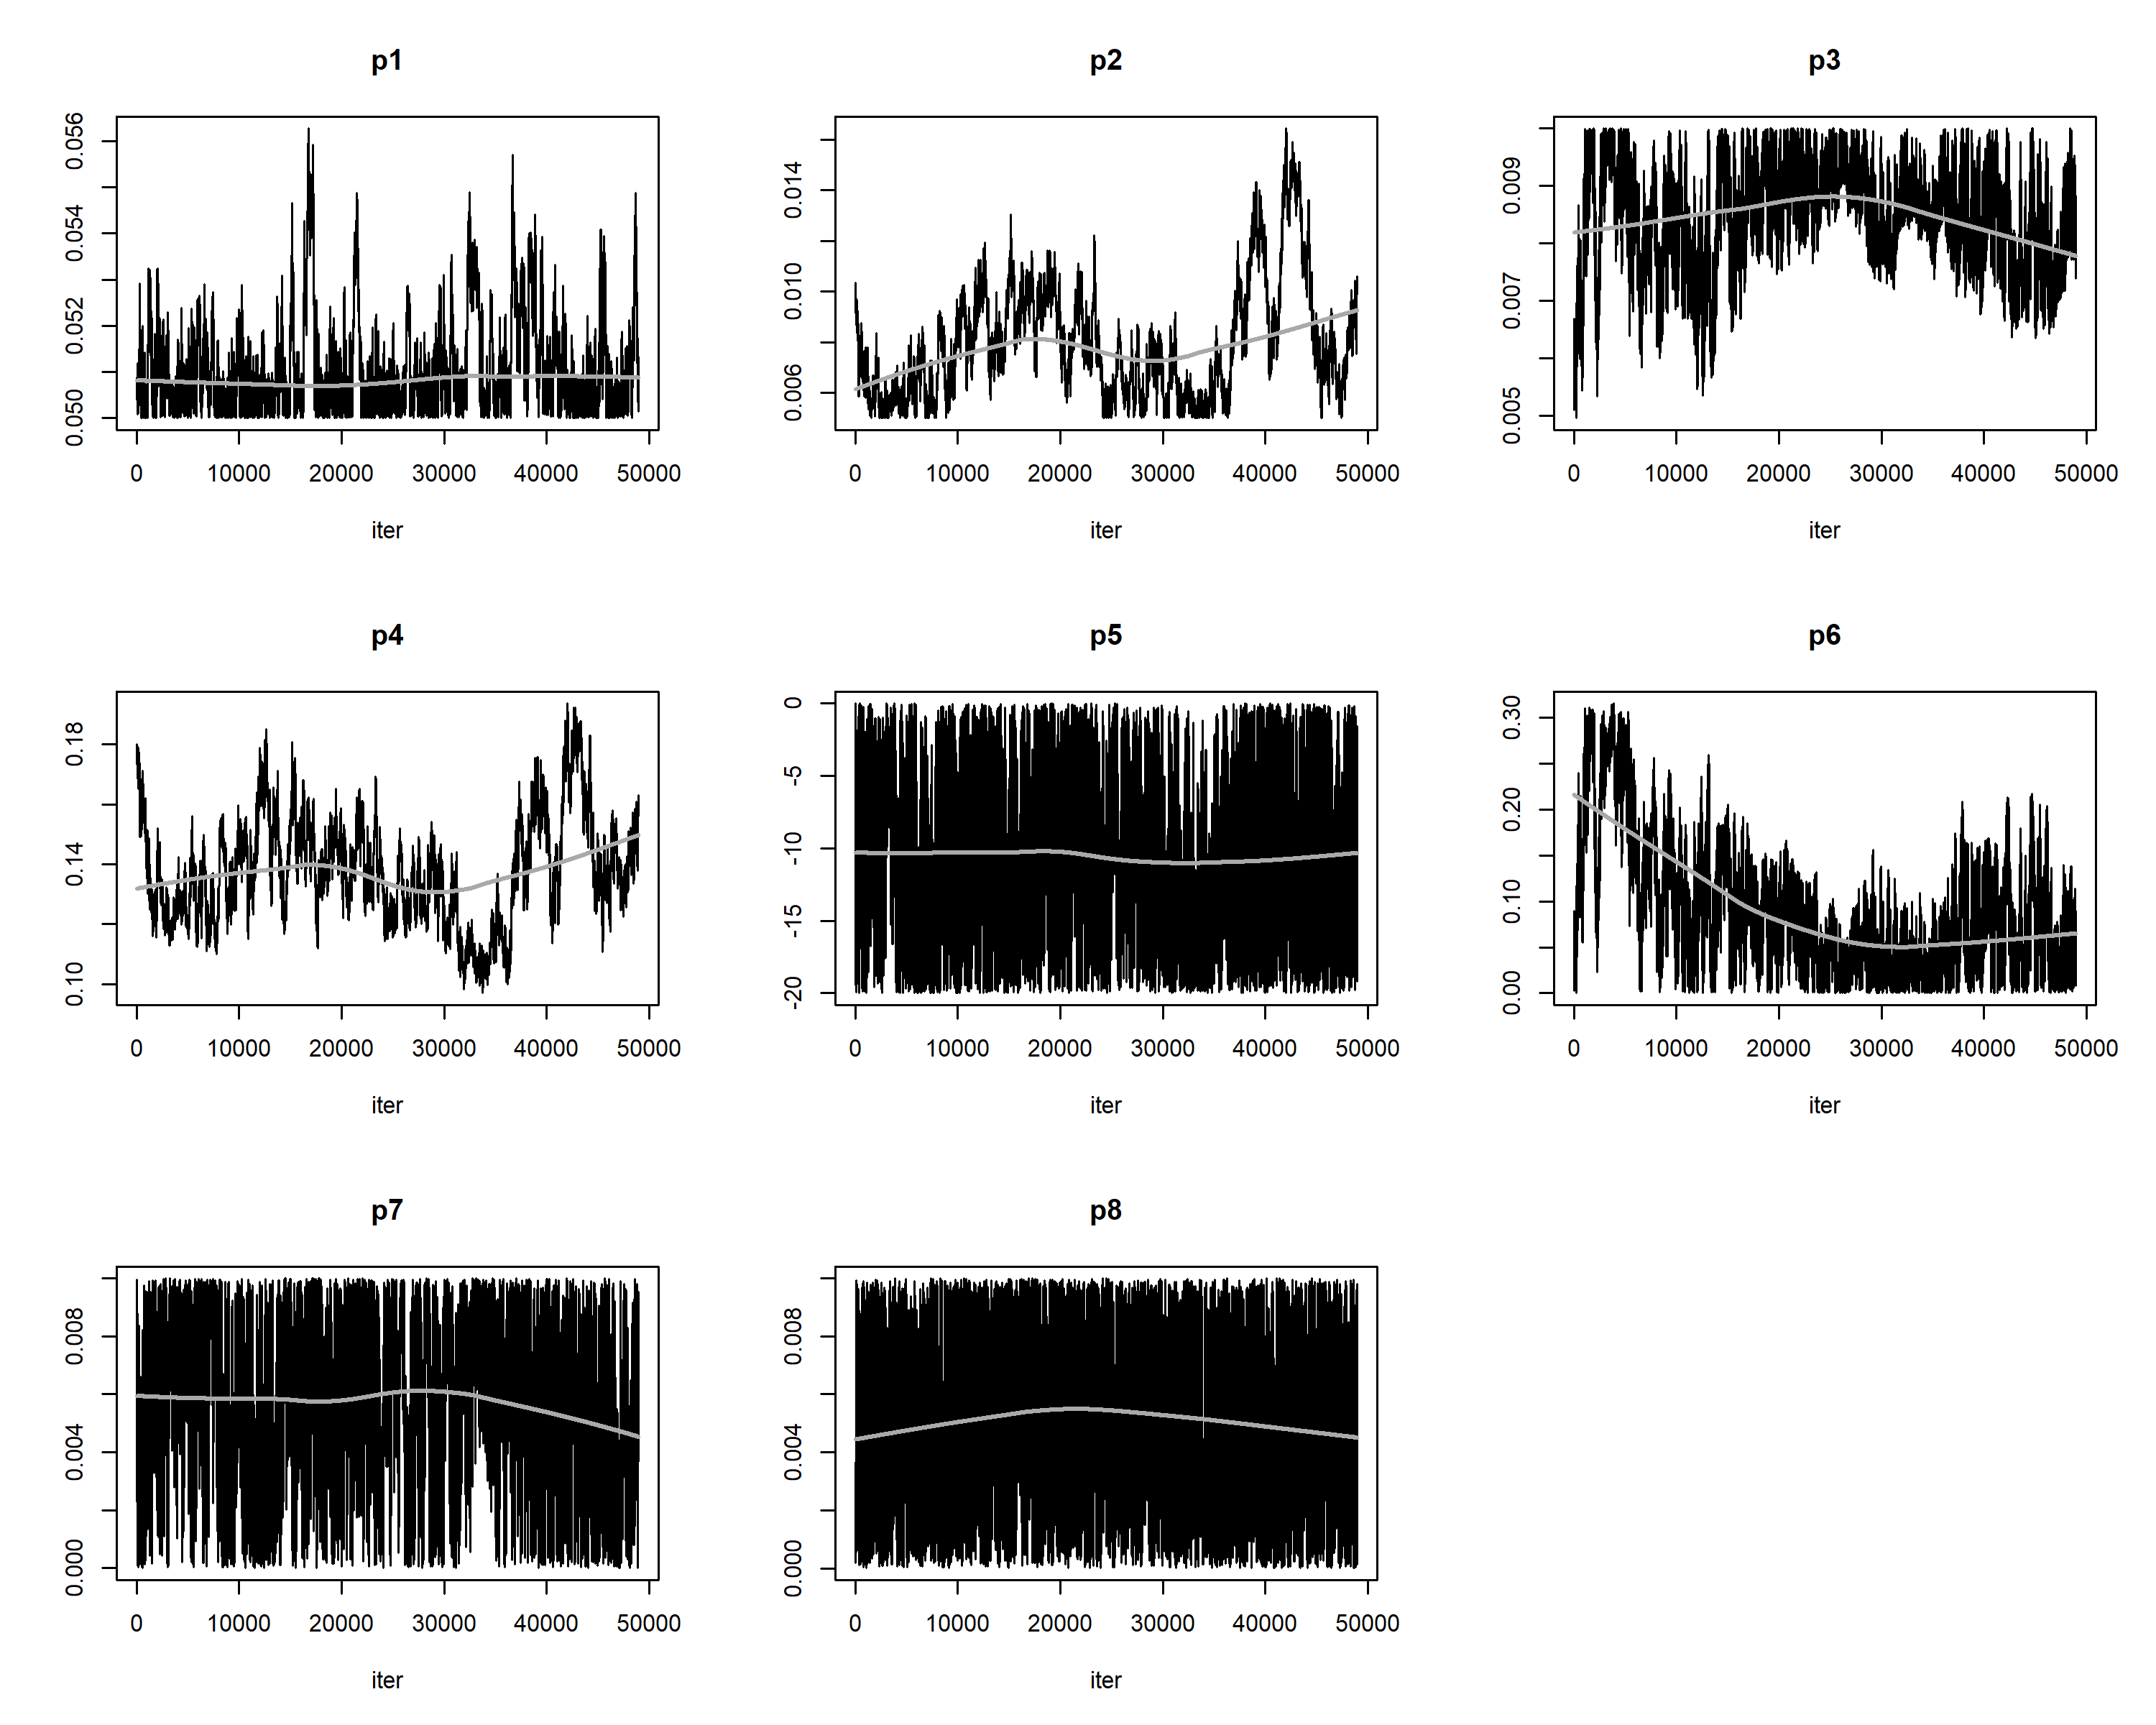
\includegraphics[width=11cm]{images/convergence_plot.png}
\caption{MCMC convergence diagnostics (trace plots). Trace plots show the evolution of sampled parameter (p) values across iterations
for each MCMC chain, where p1-p6 represent $k_f$, $k_i$, $k_s$ (fast, intermediate and slow pool decomposition rates), $a21$ (coefficient indicating proportion of C transfer from fast to slow pool), $\text{F0}_{ib}$ (a value that is subtracted from initial bulk radiocarbon measurement to find the initial intermediate radiocarbon value), $a32$ (transfer coefficient from intermediate to slow pool), $a41$ and $a42$ (transfer from fast and intermediate pools to the "loss" pool). Stable, well-mixed chains with no visible trends or drifts indicate convergence to the stationary posterior distribution.
Overlapping trajectories between chains suggest good mixing and reliable exploration of the parameter space.}
\end{figure}
\clearpage

  %%fig A4
\begin{figure}[t]
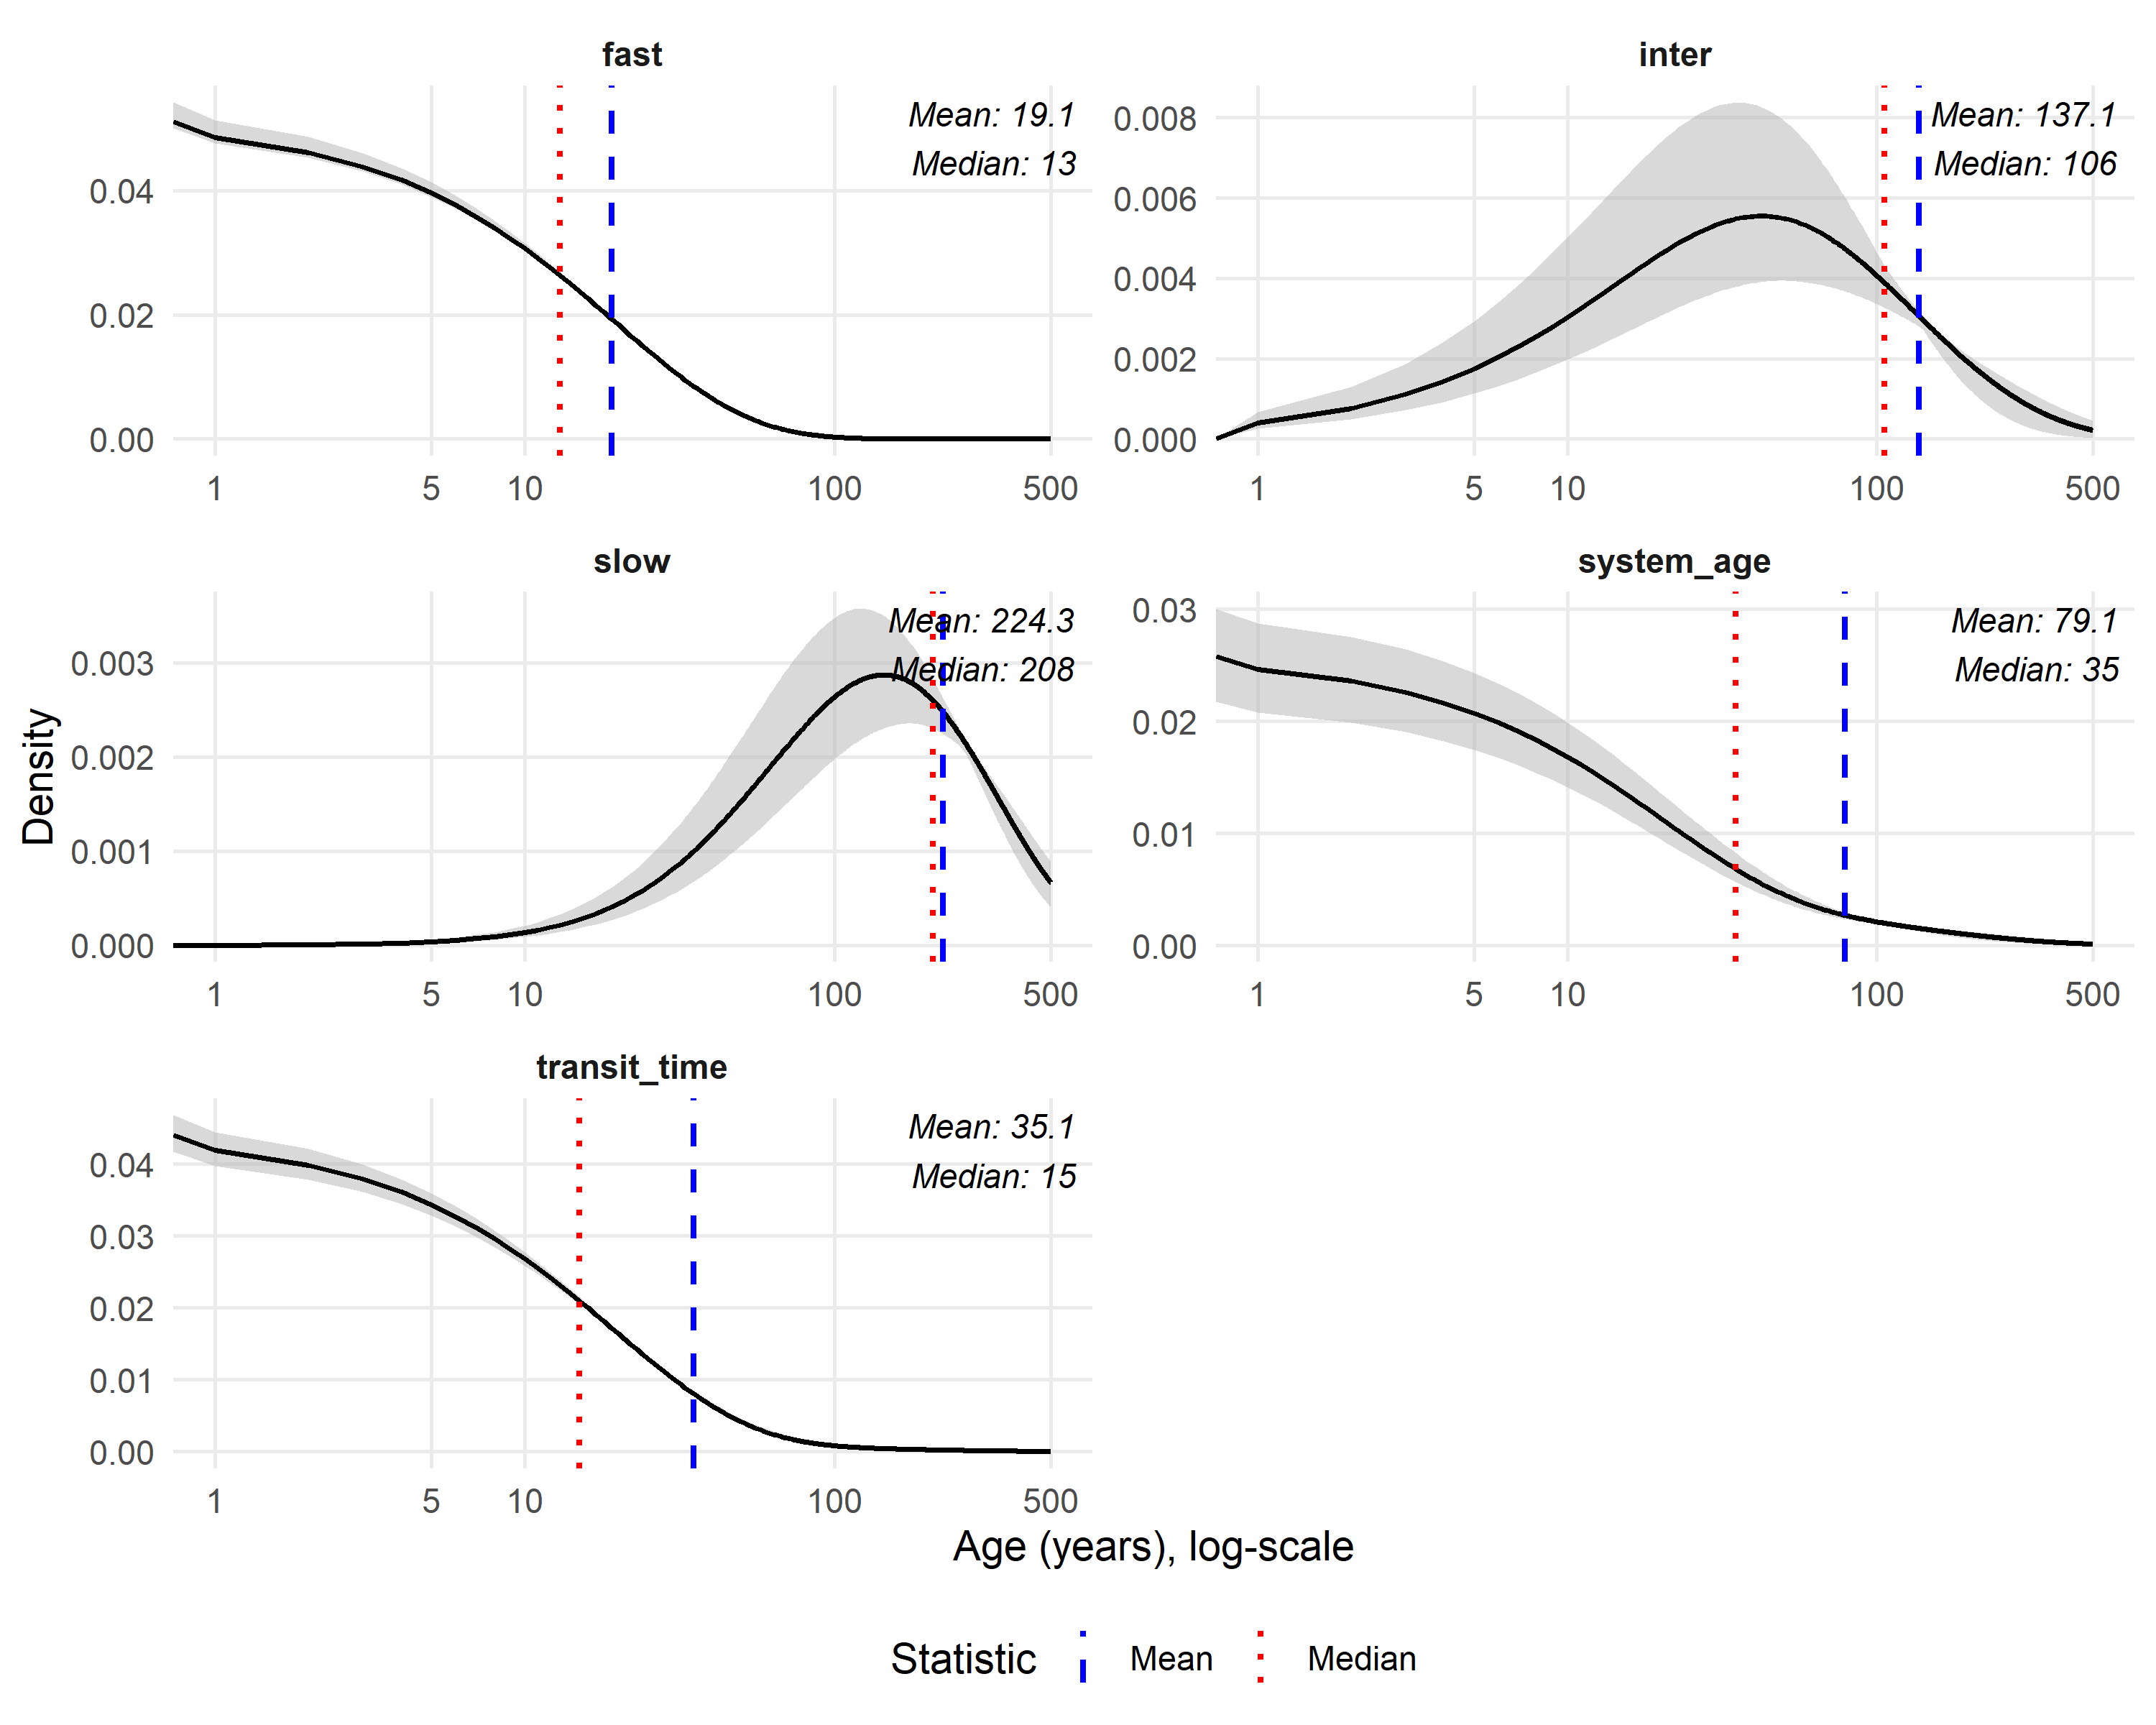
\includegraphics[width=12cm]{images/plot_log_age_tt.png}
\caption{Soil system and organic matter pool age distribution and soil transit time distribution with posterior mean density as a central
estimate and shaded regions representing the 95\% confidence interval across parameter uncertainty. Vertical lines indicate the densityweighted mean (blue dashed) and median (red dotted) ages.}
\label{figure:A2}
\end{figure}
\clearpage
  
  %%fig A5
\begin{figure}[t]

\includegraphics[width=12cm]{images/flux_plot.png}
\caption{Modeled steady-state SOM carbon flux partitioning among respiratory losses, stabilization pathways, and external export.}
\label{figure:A3}
\end{figure}

\clearpage

\noappendix   

\bibliographystyle{copernicus}
\bibliography{references.bib}

\end{document}